\documentclass[border=10pt]{standalone}

\usepackage{tikz}
\usepackage{tikzsymbols}
\usetikzlibrary{calc,patterns,shapes.geometric}

\def\centerarc[#1](#2)(#3:#4:#5){\draw[#1] ($(#2)+({#5*cos(#3)},{#5*sin(#3)})$) arc (#3:#4:#5);}

\begin{document}
	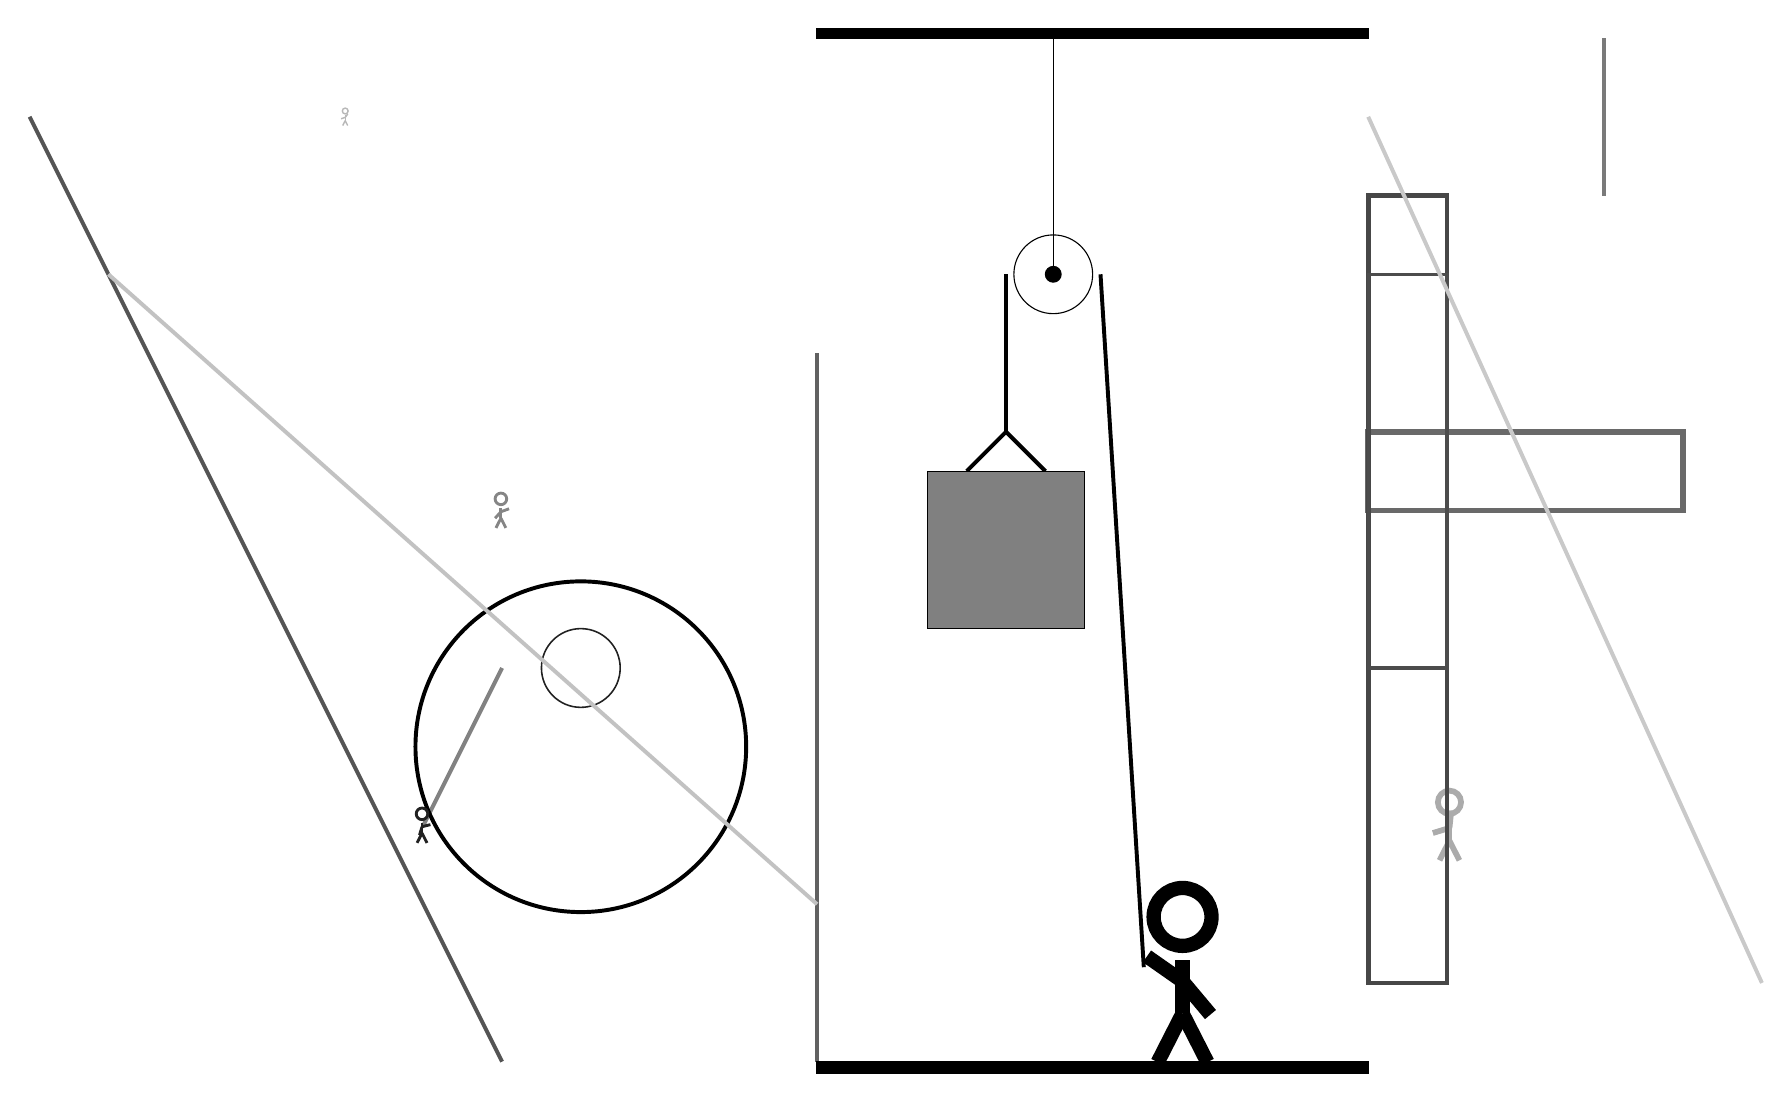
\begin{tikzpicture}
		%%%%% START %%%%%
		
		\draw[fill=black] (-2, 10) rectangle (5, 10.125);
		
		\draw (1, 7) circle (0.5);
		\draw[fill=black] (1, 7) circle (0.1);
		\draw (1, 10) -- (1, 7);
		
		\node[line width=0.5mm, color=black!33] at (6, 0) {\Strichmaxerl[4][17][84]};
		
		\draw [line width=0.2mm, color=black!87](-5, 2) circle (0.5);
		\node[line width=0.6mm, color=black!28] at (-8, 9) {\Strichmaxerl[1][18][54]};
		\draw[line width=0.7mm, color=black!59] (5, 4) rectangle (9, 5);
		\draw[line width=0.5mm, color=black!49](-6, 2) -- (-7, 0);
		\draw[line width=0.6mm, color=black!72] (6, 8) rectangle (5, -2);
		\draw[line width=0.5mm, color=black!62](-2, -3) -- (-2, 6);
		
		\draw [line width=0.5mm, color=black!100](-5, 1) circle (2.1);
		\node[line width=0.4mm, color=black!87] at (-7, 0) {\Strichmaxerl[2][73][14]};
		\draw[line width=0.5mm, color=black!67](-6, -3) -- (-12, 9);
		\draw[line width=0.5mm, color=black!24](-2, -1) -- (-11, 7);
		\node[line width=0.3mm, color=black!48] at (-6, 4) {\Strichmaxerl[2][48][20]};
		\draw[line width=0.5mm, color=black!52](8, 10) -- (8, 8);
		\draw[line width=0.4mm, color=black!70] (6, 2) rectangle (5, 7);
		\draw[line width=0.5mm, color=black!21](10, -2) -- (5, 9);
		
		\draw[line width=0.5mm] (-0.1, 4.5) -- (0.4, 5.0) -- (0.9, 4.5);
		\draw[fill=black!50] (-0.6, 4.5) rectangle (1.4, 2.5);
		
		\draw[line width=0.5mm] (0.4, 7) -- (0.4, 5.0);
		\centerarc[line width=0.5mm](1, 7)(0:180:0.6);
		\draw[line width=0.5mm](1.6, 7) -- (2.15, -1.8);
		
		\node at (2.6, -1.9) {\Strichmaxerl[10][-35][-50]};
		
		\draw[fill=black] (-2, -3) rectangle (5, -3.15);
		
		%%%%% END %%%%%
	\end{tikzpicture}
\end{document}